\chapter{Subspaces, Projection Operators, and Measurement as Entanglement}

This chapter follows Leonard Susskind's sixth lecture in the Quantum Entanglement series, curated by LazyingArt LLC. The order matters. The lecture begins in the afterpressure of Bell's theorem, where locality and entanglement are still the live issue in the room; then it deliberately backs up and repairs the mathematics of subspaces and projection operators; only after that does it return to the promised subject, namely the relation among measurement, collapse of the wave packet, and entanglement. The payoff is not a slogan but a mechanism: a measurement is the establishment of entanglement between a system and an apparatus, and it is precisely the recording of that information that destroys interference.

\section{Opening Motivation: Entanglement, Locality, and Measurement}

The lecture does not open with a neat new beginning. It opens with a question left over from the Bell discussion: if one member of an entangled pair is measured, is there some exchange, some message, some detectable event at the other side? Susskind's answer is operational and uncompromising. Nothing detectable happens at the far side. No usable signal arrives there. One may act on one member of an entangled pair, even rotate its spin locally with a magnetic field, and the detailed form of the joint state may change, but the distant system remains entangled with whatever system lives here.

That already forces a broader notion of what counts as the system. If one member of an entangled pair falls into a black hole, the other does not cease to be entangled; rather, it becomes entangled with the larger system containing the black hole degrees of freedom and, later, the emitted radiation. Susskind immediately domesticates the same point with the bathtub example. Drop one member of an entangled pair into a tub and let it mix violently with the water. The distant particle is no longer neatly entangled with one identifiable partner. It is entangled with the state of the bathtub.

This is not only a story about persistence. It is also a story about reversibility. If interaction can create entanglement, then interaction can, in principle, undo it. Disentanglement is possible, but only when the systems come back into contact and interact again. Anything that can happen one way can happen the other way.

The room then asks exactly the question that drives the rest of the lecture. Suppose the two particles are entangled and we measure them. Are they still entangled afterwards, or does measurement kick them out? Susskind answers that measurement does kick them out, or at least can. But he refuses to answer too quickly. Instead he states the real target of the evening: the relation among observation, collapse of the wave packet, and entanglement. Then he says, in effect, that before we can get there he must first clean up the mathematics of projection operators and subspaces.

\section{Dimension, Linear Dependence, and Orthonormal Bases}

We therefore stay, for the moment, with finite-dimensional vector spaces equipped with bras, kets, and an inner product. Susskind begins as elementarily as possible. He does not define dimension by counting components in a column vector. He defines it abstractly: the dimension of a vector space is the maximum number of linearly independent vectors that can be found in it.

Thus a collection \(\{|v_i\rangle\}\) is linearly independent when the relation
\begin{equation}
\sum_i c_i |v_i\rangle = 0
\end{equation}
forces all the coefficients \(c_i\) to vanish. Equivalently, none of the vectors can be written as a linear combination of the others.

It is crucial here that orthogonality is not the same thing as independence. In three dimensions one may have three vectors that are not orthogonal at all and yet are linearly independent. What matters is whether one of them can be built from the other two. On the other hand, in a two-dimensional plane any third vector in that plane must be linearly dependent on the first two.

\begin{figure}[htbp]
\centering

\includegraphics[width=0.56\textwidth]{lecture_06_figure_02.png}
\caption{Three vectors drawn on the board. The lecture uses this sketch to separate the idea of orthogonality from the idea of linear independence, and then to emphasize that in a plane a third vector is dependent on the first two.}
\end{figure}

\begin{figure}[htbp]
\centering
\begin{tikzpicture}[scale=1.2]
\draw[->] (0,0) -- (2.3,0);
\draw[->] (0,0) -- (2.0,2.0);
\draw[->] (0.35,0.95) -- (1.05,1.45);
\fill (0,0) circle (1.2pt);
\end{tikzpicture}
\caption{A minimal reconstruction of the board sketch. The exact coefficient relation is not fixed by the frame alone; the geometric point is that in a two-dimensional plane a third vector is not independent.}
\end{figure}

This is the point of the sketch. If the space is two-dimensional, the maximum number of linearly independent vectors is two. If the space is three-dimensional, it is three. More generally, if the space has dimension \(d\), then, given an inner product, one can find \(d\) mutually orthogonal unit vectors spanning it. Those are basis vectors. Susskind explicitly says he will not prove that theorem here. He only wants the conclusion: once such a basis exists, every vector in the space can be expanded in it.

\subsection{Question \& Answer: Are spatial degrees of freedom the same thing as the dimension of the state space?}

No. A particle moving in ordinary three-dimensional space has three spatial degrees of freedom in the mechanical sense, but that fact does not determine the dimension of its space of states. Those are different notions. A particle moving in a room has three spatial directions available to it, but an enormous number of orthogonal possible states. The lecture stays in finite-dimensional toy models only because that is the cleanest place to see the logic of subspaces and projectors.

\section{Basis Expansion, Dyads, and the Resolution of Identity}

Now choose an orthonormal basis \(\{|n\rangle\}\), with \(n=1,\dots,d\). The blackboard at this point is especially clear and compact:

\begin{figure}[htbp]
\centering

\includegraphics[width=0.62\textwidth]{lecture_06_figure_03.png}
\caption{Orthonormal basis and expansion of an arbitrary state.}
\end{figure}

We write
\begin{align}
\langle m|n\rangle &= \delta_{mn}, \\
|\psi\rangle &= \sum_n a_n |n\rangle.
\end{align}
Here \(\delta_{mn}\) is the Kronecker delta: it is \(1\) when \(m=n\) and \(0\) otherwise.

\paragraph{Worked derivation.} The coefficients are recovered by projecting onto the basis. Multiply by \(\langle m|\) on the left:
\begin{align}
\langle m|\psi\rangle
  &= \sum_n a_n \langle m|n\rangle \\
  &= \sum_n a_n \delta_{mn} \\
  &= a_m.
\end{align}
So the coefficients are simply
\begin{equation}
a_m = \langle m|\psi\rangle.
\end{equation}
At this point the lecture pauses to note that the coefficient is just an ordinary complex number, so one may place it on either side of the ket without changing anything.

If we substitute the coefficient back into the expansion, we get
\begin{equation}
|\psi\rangle = \sum_n |n\rangle \langle n|\psi\rangle.
\end{equation}
This suggests that the object \(|n\rangle\langle n|\), and more generally \(|a\rangle\langle b|\), ought to be read as an operator. That is exactly the next move. A dyad acts by
\begin{equation}
\bigl(|a\rangle\langle b|\bigr)|\psi\rangle = \langle b|\psi\rangle\,|a\rangle.
\end{equation}
The bra extracts a complex number; the ket supplies the resulting direction. This is Susskind's low-tech route from vectors to operators.

Now read the previous expansion operatorially. Since
\begin{equation}
|\psi\rangle = \left(\sum_n |n\rangle\langle n|\right)|\psi\rangle
\end{equation}
for every \(|\psi\rangle\), the operator in parentheses must be the identity:
\begin{equation}
\sum_n |n\rangle\langle n| = I.
\end{equation}
This is the resolution of the identity.

The lecture briefly lingers on a useful observation. The identity operator is itself a projection operator, namely the projection onto the whole space. Every vector is an eigenvector of \(I\), and every eigenvalue is \(+1\). That is not a deep theorem; it is just a clean way of seeing what the identity operator means.

\section{Properties as Subspaces and Projection Operators}

With that machinery in hand, the lecture makes its central conceptual correction. A property such as \(k=\lambda\) is not, in general, one vector. It is a whole subspace.

Let \(k\) be a Hermitian observable and suppose
\begin{equation}
k|A\rangle = \lambda |A\rangle, \qquad
k|B\rangle = \lambda |B\rangle,
\end{equation}
with \(|A\rangle\) and \(|B\rangle\) linearly independent. Then any linear combination has the same eigenvalue:
\begin{align}
k\bigl(\alpha|A\rangle+\beta|B\rangle\bigr)
  &= \alpha k|A\rangle + \beta k|B\rangle \\
  &= \alpha \lambda |A\rangle + \beta \lambda |B\rangle \\
  &= \lambda\bigl(\alpha|A\rangle+\beta|B\rangle\bigr).
\end{align}
So the eigenspace for \(\lambda\) is closed under addition and scalar multiplication. It is a vector subspace.

The lecture's first concrete example is a two-spin system. The states
\begin{equation}
|ud\rangle,\qquad |uu\rangle
\end{equation}
have different values of the second spin, but the same value of the first: the first spin is up in both cases. So they span the subspace in which \(\sigma_3=+1\) for the first spin.

\begin{figure}[htbp]
\centering

\includegraphics[width=0.46\textwidth]{lecture_06_figure_04.png}
\caption{Two two-spin states with first spin up.}
\end{figure}

That is the point worth preserving: a property is not necessarily one state. It is a whole collection of states with the same eigenvalue.

To avoid the notational confusion that appears briefly on the blackboard, we shall keep capital letters \(A,B,\dots\) for particular eigenvectors and use lower-case \(a,b,\dots\) as summation indices running over an orthonormal basis of the eigensubspace. If \(\{|a\rangle\}\) is such a basis for the subspace \(k=\lambda\), then the projection operator onto that subspace is
\begin{equation}
\Pi_{k=\lambda}=\sum_a |a\rangle\langle a|.
\end{equation}
This is just the identity operator restricted to the subspace. If \(|\psi\rangle\) already lies in that subspace, the projector returns it unchanged. If \(|\psi\rangle\) lies partly outside, the projector discards the orthogonal remainder and keeps only the component inside.

\begin{figure}[htbp]
\centering

\includegraphics[width=0.44\textwidth]{lecture_06_figure_06.png}
\caption{The projected state as a vector in the eigensubspace.}
\end{figure}

\begin{figure}[htbp]
\centering
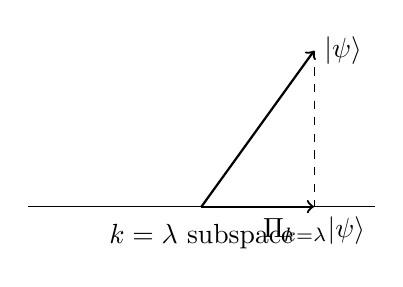
\begin{tikzpicture}[scale=1.1]
\draw (-2,0) -- (2,0);
\draw[->,thick] (0,0) -- (1.3,1.8) node[right] {$|\psi\rangle$};
\draw[dashed] (1.3,1.8) -- (1.3,0);
\draw[->,thick] (0,0) -- (1.3,0) node[below] {$\Pi_{k=\lambda}|\psi\rangle$};
\node at (0,-0.35) {$k=\lambda$ subspace};
\end{tikzpicture}
\caption{A geometric reconstruction of the lecture's point: \(\Pi_{k=\lambda}|\psi\rangle\) lies in the \(k=\lambda\) eigensubspace.}
\end{figure}

The blackboard emphasis is not only geometric. Algebraically, the projected vector satisfies
\begin{equation}
k\bigl(\Pi_{k=\lambda}|\psi\rangle\bigr)=\lambda\,\Pi_{k=\lambda}|\psi\rangle.
\end{equation}
So \(\Pi_{k=\lambda}|\psi\rangle\) really is a vector with the property \(k=\lambda\). That is what the circled board expression is trying to make visually undeniable.

\section{Probability Postulate, Compatible Properties, and the Bell Recap}

Once properties have been reinterpreted as subspaces, the probability postulate takes its cleanest form. If \(|\psi\rangle\) is normalized, then the probability that it has the property \(k=\lambda\) is
\begin{equation}
P(k=\lambda)=\langle\psi|\Pi_{k=\lambda}|\psi\rangle.
\end{equation}

\begin{figure}[htbp]
\centering

\includegraphics[width=0.58\textwidth]{lecture_06_figure_05.png}
\caption{Projector onto the \(k=\lambda\) eigensubspace. The blackboard layout already prepares the next move: sandwich the projector between \(\langle\psi|\) and \(|\psi\rangle\).}
\end{figure}

Insert the dyadic form of the projector:
\begin{align}
P(k=\lambda)
  &= \left\langle \psi \left| \sum_a |a\rangle\langle a| \right| \psi \right\rangle \\
  &= \sum_a \langle\psi|a\rangle\langle a|\psi\rangle \\
  &= \sum_a |\langle a|\psi\rangle|^2.
\end{align}
This is exactly the lecture's interpretation: the total probability for the property is the sum of the probabilities of all the orthogonal ways in which the property can occur.

For the first spin being up in a two-spin system, the relevant subspace is spanned by \(|uu\rangle\) and \(|ud\rangle\), so
\begin{equation}
\Pi_{\sigma_3=+1}=|uu\rangle\langle uu|+|ud\rangle\langle ud|.
\end{equation}
In the lecture's shorthand this is also written as
\begin{equation}
\Pi_{\sigma_3=+1}=\frac{1+\sigma_3}{2},
\end{equation}
with the identity on the second spin suppressed.

\subsection{Question \& Answer: What is the difference between an observable, a property, and a projector?}

The observable is the Hermitian operator \(k\). The property is the statement \(k=\lambda\), namely the statement that a measurement of \(k\) would certainly yield the value \(\lambda\). That property is represented not by a single vector in general, but by the eigensubspace for \(\lambda\). The projector \(\Pi_{k=\lambda}\) is then the operator that isolates that subspace, and its expectation value in the state \(|\psi\rangle\) gives the probability that the property is present.

The lecture then asks how to combine properties. Suppose we have two compatible properties, represented by commuting projectors \(P_k\) and \(P_\ell\). In the lecture's language, the AND statement is represented by the product:
\begin{equation}
\Pi_{k=\lambda\,\wedge\,\ell=\mu}=P_kP_\ell=P_\ell P_k.
\end{equation}
The logic is simple. \(P_k|\psi\rangle\) lies in the \(k=\lambda\) subspace. Because the operators commute, \(P_\ell P_k|\psi\rangle=P_kP_\ell|\psi\rangle\), so the same vector lies in the \(\ell=\mu\) subspace as well. Thus the product projects onto the simultaneous property. The corresponding probability is
\begin{equation}
P(k=\lambda,\ell=\mu)=\langle\psi|P_kP_\ell|\psi\rangle.
\end{equation}

\begin{figure}[htbp]
\centering
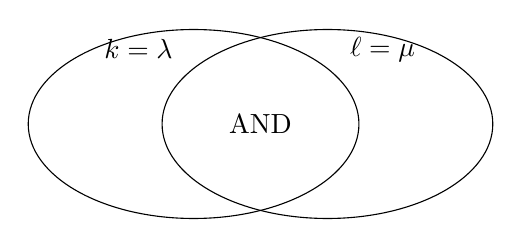
\begin{tikzpicture}[scale=1.0]
\draw (0,0) ellipse (2.1 and 1.2);
\draw (1.7,0) ellipse (2.1 and 1.2);
\node at (-0.7,0.95) {$k=\lambda$};
\node at (2.4,0.95) {$\ell=\mu$};
\node at (0.85,0) {AND};
\end{tikzpicture}
\caption{A reconstruction of the intersecting-subspace picture behind the AND statement for commuting projectors.}
\end{figure}

\begin{remark}
The lecture also treats the OR statement, in this same compatible setting, as the sum of the projectors. We keep that claim in precisely this local context and do not silently upgrade it into a more general theorem.
\end{remark}

Compatibility itself is then tied back to physical examples. In a two-spin system, any component \(\sigma_i\) of the first spin commutes with any component \(\tau_j\) of the second:
\begin{equation}
[\sigma_i,\tau_j]=0.
\end{equation}
By contrast, different components of the same spin do not commute:
\begin{equation}
[\sigma_1,\sigma_3]\neq 0.
\end{equation}
That is why one may measure one component of each of two separated spins, but not simultaneously measure two different components of the same spin.

Now Susskind revisits Bell's theorem. He does not redo last lecture's arithmetic. He rebuilds its logic in the new language. The classical inequality, in probabilistic form, is
\begin{equation}
P(A\wedge \neg B)+P(B\wedge \neg C)\ge P(A\wedge \neg C).
\end{equation}
This is a theorem of classical set logic, not of quantum mechanics. In the singlet state, spins are anti-aligned along any common axis, so a NOT statement for the first spin can be traded for the corresponding positive statement for the second. That lets one rewrite the inequality as a statement about joint properties of a two-spin system.

Suppressing identity operators on untouched factors, the single-property projectors appearing in the lecture are
\begin{equation}
\frac{1+\sigma_3}{2},\qquad
\frac{1+\frac{\tau_1+\tau_3}{\sqrt2}}{2},\qquad
\frac{1+\frac{\sigma_1+\sigma_3}{\sqrt2}}{2},\qquad
\frac{1+\tau_1}{2}.
\end{equation}
Therefore the three relevant joint projectors are
\begin{align}
\Pi_1 &= \frac{1+\sigma_3}{2}\,\frac{1+\frac{\tau_1+\tau_3}{\sqrt2}}{2}, \\
\Pi_2 &= \frac{1+\frac{\sigma_1+\sigma_3}{\sqrt2}}{2}\,\frac{1+\tau_1}{2}, \\
\Pi_3 &= \frac{1+\sigma_3}{2}\,\frac{1+\tau_1}{2}.
\end{align}
The lecture speaks of the singlet in the familiar unnormalized blackboard form
\begin{equation}
|\Psi_{\mathrm{singlet}}\rangle \propto |ud\rangle-|du\rangle.
\end{equation}
The proportionality sign is enough here. What matters for the logic is the state itself and, in particular, the relative sign, not the overall normalization. Evaluating \(\langle \Pi_1\rangle+\langle \Pi_2\rangle\) against \(\langle \Pi_3\rangle\) in the singlet state yields the violation obtained in the previous lecture. The important conclusion is the one Susskind emphasizes verbally: quantum mechanics is not classical set theory in disguise.

\section{Locality After Bell}

That Bell recap leads straight into the physical unease still hanging over the room. If the correlations are real, why can they not be used to send a signal?

\subsection{Question \& Answer: Why can’t entanglement be used to send a faster-than-light signal?}

The answer remains stubbornly operational. If the second measurement is performed only after enough time has elapsed for an ordinary light signal to travel from the first apparatus to the second, then there is no contradiction with causality. One may still wonder what mechanism carried the information, but one has not yet outrun the light cone.

The sharp Bell experiment is therefore arranged in the opposite way: the settings and outcomes are chosen so that no light signal could have crossed from one wing of the experiment to the other in time. That is what makes the result strange without turning it into a signaling device. The correlations remain, but no usable message has been transmitted. When one says that any hidden-variable account reproducing these facts must be nonlocal, one means precisely that it would need some influence not bounded by the speed of light.

This discussion does not close the lecture; it clears the ground for the next pivot. Bell has taught us that quantum mechanics is not classical logic, but the next question is different. What is a measurement, operationally and mathematically, and how does it enter the story of interference?

\section{Finite-State Two-Slit, Interference, and Measurement as Entanglement}

The lecture now changes model. Susskind turns to the two-slit experiment, but he immediately simplifies it into a finite-state problem so that the same vector-space technology can be used without bringing in the full machinery of continuum wave mechanics. He even says, in effect, that this is still the two-slit experiment, only stripped down to a small set of basis states.

There is a source state \(|0\rangle\), two slit states \(|1\rangle\) and \(|-1\rangle\), and a set of screen states \(|n\rangle\). These \(|n\rangle\) are orthonormal because distinct screen positions are distinct configurations. The lecture explicitly chooses not to track normalization carefully here. Unitarity is postponed. What matters at this stage is linearity.

\begin{figure}[htbp]
\centering
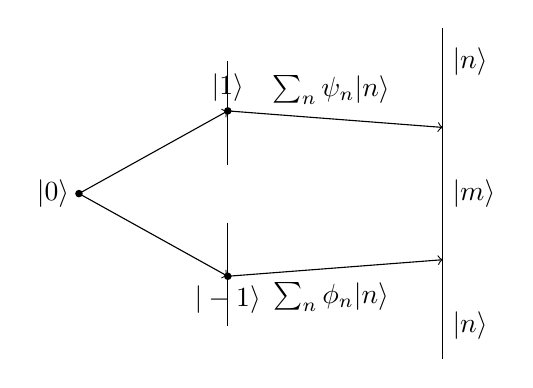
\begin{tikzpicture}[scale=1.05]
\fill (0,0) circle (1.3pt);
\node[left] at (0,0) {$|0\rangle$};

\draw (1.8,1.6) -- (1.8,0.35);
\draw (1.8,-0.35) -- (1.8,-1.6);
\fill (1.8,1) circle (1.3pt);
\fill (1.8,-1) circle (1.3pt);
\node[above] at (1.8,1) {$|1\rangle$};
\node[below] at (1.8,-1) {$|-1\rangle$};

\draw (4.4,2.0) -- (4.4,-2.0);
\node[right] at (4.4,1.6) {$|n\rangle$};
\node[right] at (4.4,0.0) {$|m\rangle$};
\node[right] at (4.4,-1.6) {$|n\rangle$};

\draw[->] (0,0) -- (1.8,1);
\draw[->] (0,0) -- (1.8,-1);
\draw[->] (1.8,1) -- (4.4,0.8);
\draw[->] (1.8,-1) -- (4.4,-0.8);

\node at (3.05,1.25) {$\sum_n \psi_n |n\rangle$};
\node at (3.05,-1.25) {$\sum_n \phi_n |n\rangle$};
\end{tikzpicture}
\caption{A finite-state version of the two-slit experiment: the source state \(|0\rangle\), the two slit states \(|1\rangle\) and \(|-1\rangle\), and the screen basis \(|n\rangle\).}
\end{figure}

By symmetry the source evolves to an equal-amplitude superposition of the two slit states:
\begin{equation}
|0\rangle \longrightarrow |1\rangle+|-1\rangle.
\end{equation}
Now let the upper slit state evolve to
\begin{equation}
|1\rangle \longrightarrow \sum_n \psi_n |n\rangle,
\end{equation}
and the lower slit state to
\begin{equation}
|-1\rangle \longrightarrow \sum_n \phi_n |n\rangle.
\end{equation}
The arrows here mean time evolution, not equality of states at the same instant. By linearity,
\begin{equation}
|1\rangle+|-1\rangle \longrightarrow \sum_n (\psi_n+\phi_n)|n\rangle.
\end{equation}
That is the key rule. Amplitudes add before probabilities are formed.

The probability of arrival at the screen site \(m\) is therefore
\begin{align}
P_m &= |\psi_m+\phi_m|^2 \\
    &= |\psi_m|^2 + |\phi_m|^2 + \psi_m^*\phi_m + \phi_m^*\psi_m.
\end{align}
The first two terms are what classical reasoning would have produced. The last two are the interference terms.

At the symmetric point on the screen, call it \(m=0\), symmetry suggests \(\psi_0=\phi_0\). Then
\begin{equation}
P_0 = |\psi_0+\phi_0|^2 = |2\psi_0|^2 = 4|\psi_0|^2.
\end{equation}
Both slits open produce four times the one-slit probability at that point, not twice. This is constructive interference.

Now insert a phase shift so that \(\phi_0=-\psi_0\). Then
\begin{equation}
P_0 = |\psi_0-\psi_0|^2 = 0.
\end{equation}
Each slit by itself permits arrival at that point, but opening both together can make arrival there impossible. This is destructive interference. Susskind explicitly dwells on how odd this is: for his money it is as strange as Bell.

One electron, of course, produces only one hit. The interference pattern is the accumulated distribution obtained from many repetitions of the experiment, one particle at a time. This too is part of the lecture's rhythm: a single event is only a blip; the pattern is statistical.

Now we introduce the apparatus. There is one additional two-state system, a spin initially in the state \(|d\rangle\). If the electron goes through the upper slit, it flips that spin to \(|u\rangle\). If it goes through the lower slit, it leaves it unchanged. The initial composite state is \(|0,d\rangle\), and the first update rule becomes
\begin{equation}
|0,d\rangle \longrightarrow |1,u\rangle + |-1,d\rangle.
\end{equation}
That one line is the whole meaning of measurement in the lecture. The position of the electron has become entangled with the record stored in the apparatus.

\begin{figure}[htbp]
\centering
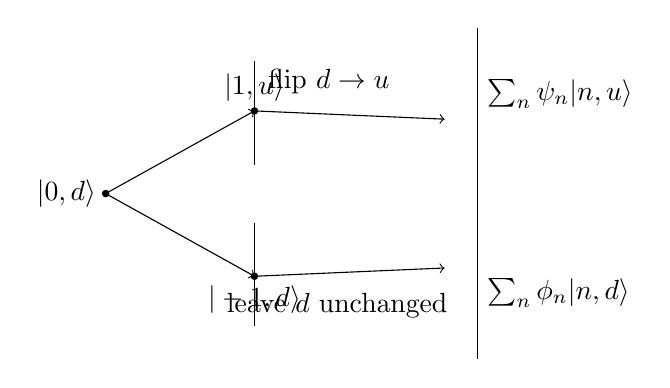
\begin{tikzpicture}[scale=1.05]
\fill (0,0) circle (1.3pt);
\node[left] at (0,0) {$|0,d\rangle$};

\draw (1.8,1.6) -- (1.8,0.35);
\draw (1.8,-0.35) -- (1.8,-1.6);
\fill (1.8,1) circle (1.3pt);
\fill (1.8,-1) circle (1.3pt);
\node[above] at (1.8,1) {$|1,u\rangle$};
\node[below] at (1.8,-1) {$|-1,d\rangle$};

\draw (4.5,2.0) -- (4.5,-2.0);
\node[right] at (4.5,1.2) {$\sum_n \psi_n |n,u\rangle$};
\node[right] at (4.5,-1.2) {$\sum_n \phi_n |n,d\rangle$};

\draw[->] (0,0) -- (1.8,1);
\draw[->] (0,0) -- (1.8,-1);
\draw[->] (1.8,1) -- (4.1,0.9);
\draw[->] (1.8,-1) -- (4.1,-0.9);

\node at (2.7,1.35) {flip \(d\to u\)};
\node at (2.8,-1.35) {leave \(d\) unchanged};
\end{tikzpicture}
\caption{Measurement as entanglement with a detector spin. The upper path flips the apparatus spin; the lower path leaves it untouched.}
\end{figure}

Assume, as the lecture does, that nothing further happens to the spin during the journey to the screen. Then
\begin{align}
|1,u\rangle &\longrightarrow \sum_n \psi_n |n,u\rangle, \\
|-1,d\rangle &\longrightarrow \sum_n \phi_n |n,d\rangle.
\end{align}
Therefore the final state with both slits open is
\begin{equation}
|\Psi_{\mathrm{final}}\rangle
  = \sum_n \psi_n |n,u\rangle + \sum_n \phi_n |n,d\rangle.
\end{equation}
This is not a superposition of states of one electron alone. It is an entangled state of electron and apparatus.

The cleanest way to compute the arrival probability at the site \(m\) is to use the projector onto that site on the electron subsystem:
\begin{equation}
\Pi_m = |m\rangle\langle m|\otimes I_{\mathrm{spin}}.
\end{equation}
Applying \(\Pi_m\) to the final state gives
\begin{equation}
\Pi_m |\Psi_{\mathrm{final}}\rangle
= |m\rangle\bigl(\psi_m|u\rangle+\phi_m|d\rangle\bigr).
\end{equation}
So the probability of arrival at \(m\) is
\begin{align}
P_m
  &= \langle \Psi_{\mathrm{final}}|\Pi_m|\Psi_{\mathrm{final}}\rangle \\
  &= \bigl(\psi_m^*\langle u|+\phi_m^*\langle d|\bigr)
     \bigl(\psi_m|u\rangle+\phi_m|d\rangle\bigr) \\
  &= |\psi_m|^2 + |\phi_m|^2
     + \psi_m^*\phi_m\langle u|d\rangle
     + \phi_m^*\psi_m\langle d|u\rangle.
\end{align}
But the record states are orthogonal:
\begin{equation}
\langle u|d\rangle=0.
\end{equation}
Hence the cross terms vanish:
\begin{equation}
P_m = |\psi_m|^2 + |\phi_m|^2.
\end{equation}
That is the lecture's mathematical punchline. Once which-path information is recorded, interference disappears and probabilities add in the classical way.

\subsection{Question \& Answer: What is the difference between a one-system superposition and a two-system entangled state?}

A state such as
\begin{equation}
|1\rangle+|-1\rangle
\end{equation}
is a superposition of states of one system. There is only the electron, and it is in a linear combination of two position states.

A state such as
\begin{equation}
|1,u\rangle+|-1,d\rangle
\end{equation}
is different in kind. Now there are two systems, the electron and the detector spin, and the state is not a statement about either subsystem separately. It correlates them. Looking at the spin tells us something about the path, and that is exactly why Susskind says that a measurement is the establishment of entanglement between system and apparatus.

The lecture closes by widening that claim. A deliberately built detector is not the only recorder. An atom near a slit, a bit of gas, a thermal environment, any additional degree of freedom that becomes sufficiently entangled with the electron can destroy the interference pattern. If the environmental record states are fully distinguishable, the interference is fully destroyed. If they overlap only partially, the interference is only partially destroyed. Susskind points toward that intermediate regime, but he does not develop its quantitative formalism here.

\section{Summary}

The lecture's mathematical spine is now plain. A property is represented, in general, not by a single state but by a subspace. The projector onto that subspace is built from an orthonormal basis of it, and the probability of the property is the expectation value of that projector. Compatible properties are combined, in the lecture's language, by multiplying commuting projectors. The same vector-space technology then reappears in the two-slit problem: without a record, amplitudes add and interference appears; with a record, the electron becomes entangled with an apparatus, the record states are orthogonal, the cross terms vanish, and probabilities add instead. This is the lecture's version of collapse: not an extra principle floating outside the formalism, but the disappearance of interference when information about the alternatives has been deposited somewhere in the world.